% % % Headers and definitions
\documentclass[10pt]{article}

\usepackage{setspace}
\usepackage{graphicx} % some graphics functions I use 
\usepackage{geometry}
\usepackage{fontspec} 
\usepackage{wrapfig}
\setmainfont{Times New Roman}

\doublespacing
\geometry{lmargin=1in, rmargin=0.5in, tmargin=1in, bmargin=0.75in}
\begin{document}

\pagenumbering{gobble} % Turn off page numbering for titles and tables

% Title and author
\Large{\center{\textbf{{Nick Levesque\\
April 7, 2015\\
ECE 331\\}}}}

\pagenumbering{arabic}
\large
% % % % % % % % % % % % % % %
% Introduction section
\section{Introduction}

\noindent This report describes in detail the design, testing, and validation of the RGB LED kernel module. The module takes three unsigned integers as input, and passes color values to an XMega32E5 on an external board, which drives the RGB LED with pulse-width modulation (PWM) . This module was designed so that multiple processes can open the associated device driver special file simultaneously, with locking used to limit writes to the external board to one process at a time. It is designed for use with all official models of the Raspberry Pi, up to and including the Raspberry Pi 2. 


% % % % % % % % % % % % % % %
% Design and analysis section
\section{Design}
In this section the design details, decisions, and the engineering rationale behind them are discussed.
\subsection{RGB Data}
\noindent To pass color data to the XMega, eleven bits are sent over three GPIO pins (thirty-three total bits in a sequence), with a fourth pin used as a clock. The most significant bits are sent first. In the module's initialization function, these pins are requested from the system and set as outputs with an initial value of zero. The kernel module is passed a struct containing three unsigned integers via an ioctl call. These integers contain the intensity values for red, green and blue. The duty cycle of the XMega's PWM output to each LED pin is high when the LED is dim, and low when the LED is at full brightness. Taking this into account, the module's ioctl handler runs a loop, decrementing a counter, \emph{i} from its initial value of ten until it reaches zero. In each iteration of the loop, the color values are shifted right by \emph{i}. The two's complement of this result is bitwise-ANDed with one, with the relevant GPIO pin being set high if the result is one. The ioctl handler sets the clock high, sets the pins to zero, sets the clock low, then continues looping until finished the sequence.


\subsection{Locking}
\noindent
\begin{wrapfigure}{o}{0.45\textwidth}
    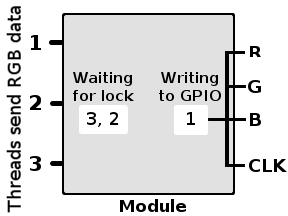
\includegraphics[width=0.45\textwidth]{figure1}
  \caption{Illustration of multi-thread handling}
\end{wrapfigure}
\noindent In order to handle multiple threads attempting to set the LED color simultaneously, only one thread is allowed to write its bit sequence at a time. Mutex locking is used to manage waiting threads. As shown in Figure 1, thread \#1 is currently writing to the GPIO pins, but thread \#2 and \#3 also want to write. Thread \#2 attempted to write before \#3, so it will acquire the lock as soon as \#1 releases it. Thread \#2 will then write its bit sequence, unlock the lock, and thread \#3 will acquire it.

\noindent When operating by itself, the differential amplifier produces a differential gain proportional to the difference between the inputs (Equation 1).

\noindent Always define the variables in an equation, unless previously defined. Typically you mention the equation, show the equation, THEN define the variables in the equation. When reporting numbers, always put the units right next to the numbers themselves. Don’t leave the numbers “naked.”

% % % % % % % % % % % % % % %		
% Simulations
\section{Testing and Validation}

\noindent Again, don’t forget to add a little blurb here about the section. You can say things like you did simulations in MicroCap, the resistor values needed to be adjusted in simulations, and so on. Just avoid having the section titles one right after the other. Don’t forget to put this section in past tense and third person too.

\subsection{Section Title}

\noindent So you put your simulated stuff here. Generally speaking, if you split up your circuit in a certain way in Section 2, you should report the simulations in a similar way. For example, if you were doing the common-source amplifier with the output stage, you might write Section 2.1 about the common-source amplifier and Section 2.2 about the output stage. Then, in your simulations, you would do Section 3.1 about your simulations for the common-source amplifier and Section 3.2 about the simulations for the output stage. This isn’t always the case, but it’s a good starting point if you’re stuck on how to format things.
\newline

\noindent Also, when you’re reporting simulation data, make sure the figures and graphs are clear. For example, if you have two lines on one graph, say that the blue line is voltage and the red line is current (or whatever). That way the reader knows what he/she is looking at. Also, label your axes. It sounds obvious, but a lot of people forget to do it.

\subsection{Section Title}

\noindent Don’t forget to add some discussion about your simulated results. Some people just report the results and move on without saying anything about them. It’s a nice idea to have a table comparing the calculated versus simulated results if it’s possible. However, don’t just put all of your data in tables – that’s not cool, bro.

% % % % % % % % % % % % % % %		
% Experimental Implementation
\section{Results and Conclusion}

\noindent Insert your little blurb here. You can talk about things like equipment numbers or preview the problems you encountered. It really depends on the lab. Again, use past tense and third person.

\subsection{Section Title}

\noindent As I said earlier, if you’re not sure how to break up Section 4, take a look at how you broke up Sections 2 and 3. Just make sure things are broken up in a way that makes sense. If you built a common-source (CS) amplifier with an output stage, try having one section on the CS amplifier and the other on the output stage.
\newline

\noindent I would recommend starting including the final schematic right after the first sentence or two of this section. You need to have a final schematic and this is the most logical place to put it. To make life easier, put the measured component values (e.g. resistor values) right in this final schematic. That way you can just say, “Measured component values are shown in Figure 4” instead of writing a bunch of awkward sentences about the resistor values.
\newline

\noindent When you’re describing how you made measurements, you don’t need to be too specific. For example, if you connected an oscilloscope to your circuit to measure voltage, you don’t need to say, “One probe was connected to the resistor and the other probe was connected to ground.” Just say, “An oscilloscope was used to measure the voltage across the resistor.” The reader should have enough “know-how” to understand how you connect an oscilloscope to a circuit.
\newline

\noindent Oh, and before I forget, if you use an abbreviation such as MOSFET, make sure you define it before you use it. For example:
\newline

\noindent A metal-oxide semiconducting field-effect transistor (MOSFET) is popular device for use in amplifiers and integrated circuits (ICs).
\newline

\end{document}
